%%%%%%%%%%%%%%%%%%%%%%%%%%%%%%%%%%%%%%%%%%%%%%%%%%%%%%%%%%%%%%%%%%%%%%%%%%%%%%%%
%2345678901234567890123456789012345678901234567890123456789012345678901234567890
%        1         2         3         4         5         6         7         8

\documentclass[letterpaper, 10 pt, conference]{ieeeconf}  % Comment this line out
                                                          % if you need a4paper
%\documentclass[a4paper, 10pt, conference]{ieeeconf}      % Use this line for a4
                                                          % paper

\IEEEoverridecommandlockouts                              % This command is only
                                                          % needed if you want to
                                                          % use the \thanks command
\overrideIEEEmargins
% See the \addtolength command later in the file to balance the column lengths
% on the last page of the document



% The following packages can be found on http:\\www.ctan.org
%\usepackage{graphics} % for pdf, bitmapped graphics files
%\usepackage{epsfig} % for postscript graphics files
%\usepackage{mathptmx} % assumes new font selection scheme installed
%\usepackage{times} % assumes new font selection scheme installed
%\usepackage{amsmath} % assumes amsmath package installed
%\usepackage{amssymb}  % assumes amsmath package installed

\usepackage{graphicx}

\title{\LARGE \bf
Quadruped Dynamic Controller Midterm Update
}

%\author{ \parbox{3 in}{\centering Huibert Kwakernaak*
%         \thanks{*Use the $\backslash$thanks command to put information here}\\
%         Faculty of Electrical Engineering, Mathematics and Computer Science\\
%         University of Twente\\
%         7500 AE Enschede, The Netherlands\\
%         {\tt\small h.kwakernaak@autsubmit.com}}
%         \hspace*{ 0.5 in}
%         \parbox{3 in}{ \centering Pradeep Misra**
%         \thanks{**The footnote marks may be inserted manually}\\
%        Department of Electrical Engineering \\
%         Wright State University\\
%         Dayton, OH 45435, USA\\
%         {\tt\small pmisra@cs.wright.edu}}
%}

% author names are place in alphabetical order so that no suggestion of whom worked the most or the least is given.
\author{Alex Tacescu, Shreyash Shantha Kumar, Sinan Morcel and Stephen Crawford}



\begin{document}



\maketitle
\thispagestyle{empty}
\pagestyle{empty}


%%%%%%%%%%%%%%%%%%%%%%%%%%%%%%%%%%%%%%%%%%%%%%%%%%%%%%%%%%%%%%%%%%%%%%%%%%%%%%%%
% \begin{abstract}


% \end{abstract}


%%%%%%%%%%%%%%%%%%%%%%%%%%%%%%%%%%%%%%%%%%%%%%%%%%%%%%%%%%%%%%%%%%%%%%%%%%%%%%%%
\section{INTRODUCTION \& PROJECT REVIEW}
Legged robots are making great strides in the real world over the past couple of years. Boston dynamics for example are presenting working models performing complex tasks for real world applications. Our aim is to develop a 4 DOF quadruped robot inspired by agility and balancing capability of a real cat. We analyze our model by designing a dynamical model for a quadruped robot and simulating it on a robotic interface . From our project we will establish a fully parameterizable gait for our model. 

We have successfully completed the initial task of training in MATLAB 2018B along with SimMechanics, build a SimMechanics model of the body and each leg, and developed a kinematic model, as well as computing the Lagrangian of one leg (which is an important milestone in the process of dynamically modeling the robot). We plan to hit our expected goals and possibly some of our reach goals. The first task is to generate a dynamical model for each leg of the quadruped robot. Similarly, generate a dynamical model for the entire system including the body and legs. Following that, the next step is  to generate the forward kinematics and dynamics for the entire robot system.

\section{LITERATURE REVIEW}
Since dynamic modeling was an issue, we dedicated some of our reading to the part of the literature that attempted or talked about the same thing. In \cite{hardt2003dynamic}, they offer something closer to a survey of different methods to model a quadruped. They offer an example of a 2-DOF-legs robot, where they describe the state vector of such systems to have the following variables: 3 Bryant Euler angles for the orientation of the whole system, 3 variables for the position of the system, 3 variables for the linear velocity, 3 for the angular one, and the vectors corresponding to the configurations of all the legs. The control variables can only directly affect the configuration of the joints, and indirectly the others.
The dynamic model of such a system has the following familiar form
$$
\ddot{q} = M(q)^{-1}\big(B\textbf{u} - C(q,\dot{q}) - G(q) + J_c(q)^T f_c\big)
\\
0 = g_c(q),
$$
which is that of a decoupled n-link robot (more than one chain of decoupled joint variables). M is the inertia matrix, B the matrix of friction coefficient of the joints, C is the matrix that corresponds to the Coriolis and centrifugal forces and G is the gravity vector. $J_c$ is the constraint Jacobian that factors into the equation the external ground constraint forces, so that they can be considered as part of the equation. $g_c$ allows us to compute the constraint Jacobian using the equation:
$$
J_c = \frac{\partial gc}{\partial q}
$$
However, the authors continue the discussion about stability guarantees and algorithms, without dwelling too much on dynamic modeling.
\\
The authors in \cite{ferguene2009dynamic} offer a very good intuition and description about what each of the terms in the typical equation of manipulator dynamics are, which helped us formulate many of our next sub-goals for the project.

\section{PROJECT UPDATE}
\subsection{CAD Model Design} \label{sec:CAD Model Design}
When starting the project, we had a model of a quadruped from another project. This quadruped had 4 DoF (degrees of freedom) per leg like we wanted, but it had one major problem: the model complexity made modeling it very difficult. Therefore, our team decided to design a simple model in Dassault Solidworks, then import it into MATLAB Simulink. The latest model can be seen in Figure 1.
We then ported the model into MATLAB using exporting software offered by  Dassault Solidworks and we used the Simscape Multibody Simulink library in MATLAB to base the simulation of the robot.
Figure \ref{fig:cadmodel} shows the cad model. The legs are equivalent, but are given this specific pose to project our vision of how we see the cat stand in the future.
\begin{figure}[thpb]
    \parbox{\linewidth}{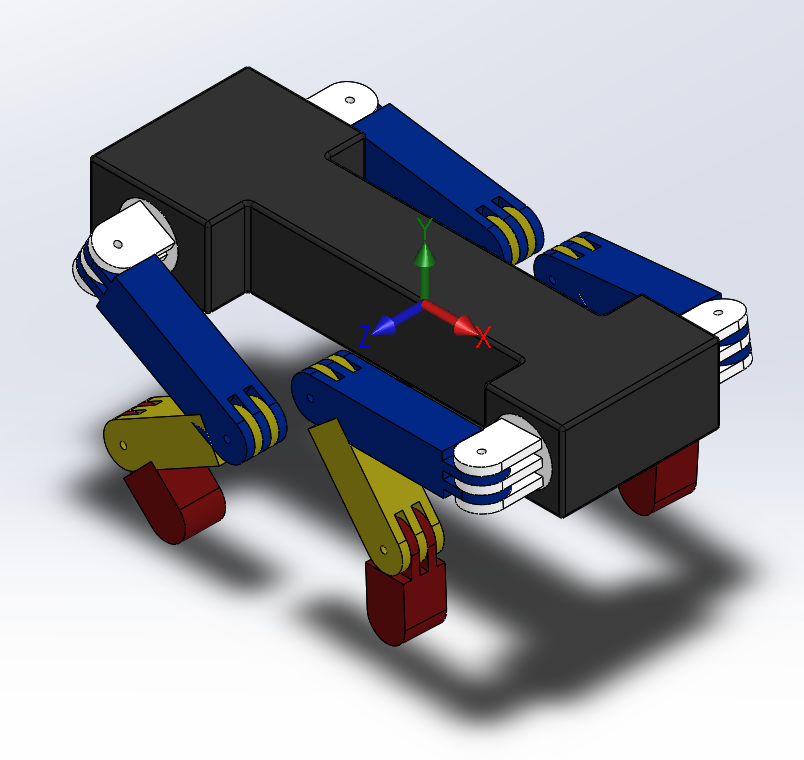
\includegraphics[width=\linewidth]{robot.png}}
    \caption{The CAD model of the simplified robot.}
    \label{fig:cadmodel}
\end{figure}

\subsection{Collision in Simulink 3D Model}
We used the Contact Forces Library to implement collision between parts of the robot and a plane we had placed underneath the robot. we used primitives called Sphere-to-plane collision blocks, which allow us to model a sphere to plane collision in SimuLink. However, without any control inputs on the legs we can't keep the legs straight to demonstrate a standing behavior of the quadruped. We did achieve a dangling pose and a crashing one for the robot, though.

Aiming to fully constraining the model (adding self-collision and body-plane collision) would send us off on a path that may derail us from reaching our reach goal. Figure \ref{fig:collision} shows an older model colliding with the floor.
\begin{figure}[thpb]
    \parbox{\linewidth}{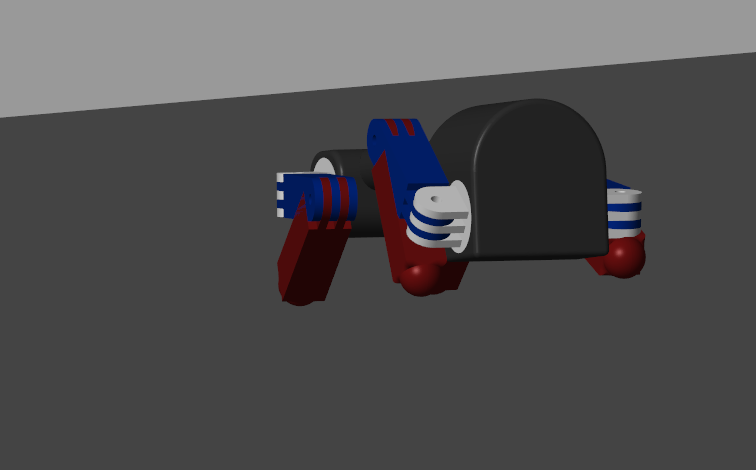
\includegraphics[width=\linewidth]{ContactModel.png}}
    \caption{The cat crashing into the floor after falling from a height.}
    \label{fig:collision}
\end{figure}

\subsection{DH-Parameters and Validation} \label{sec:dhparams}
\begin{figure}[thpb]
    \parbox{\linewidth}{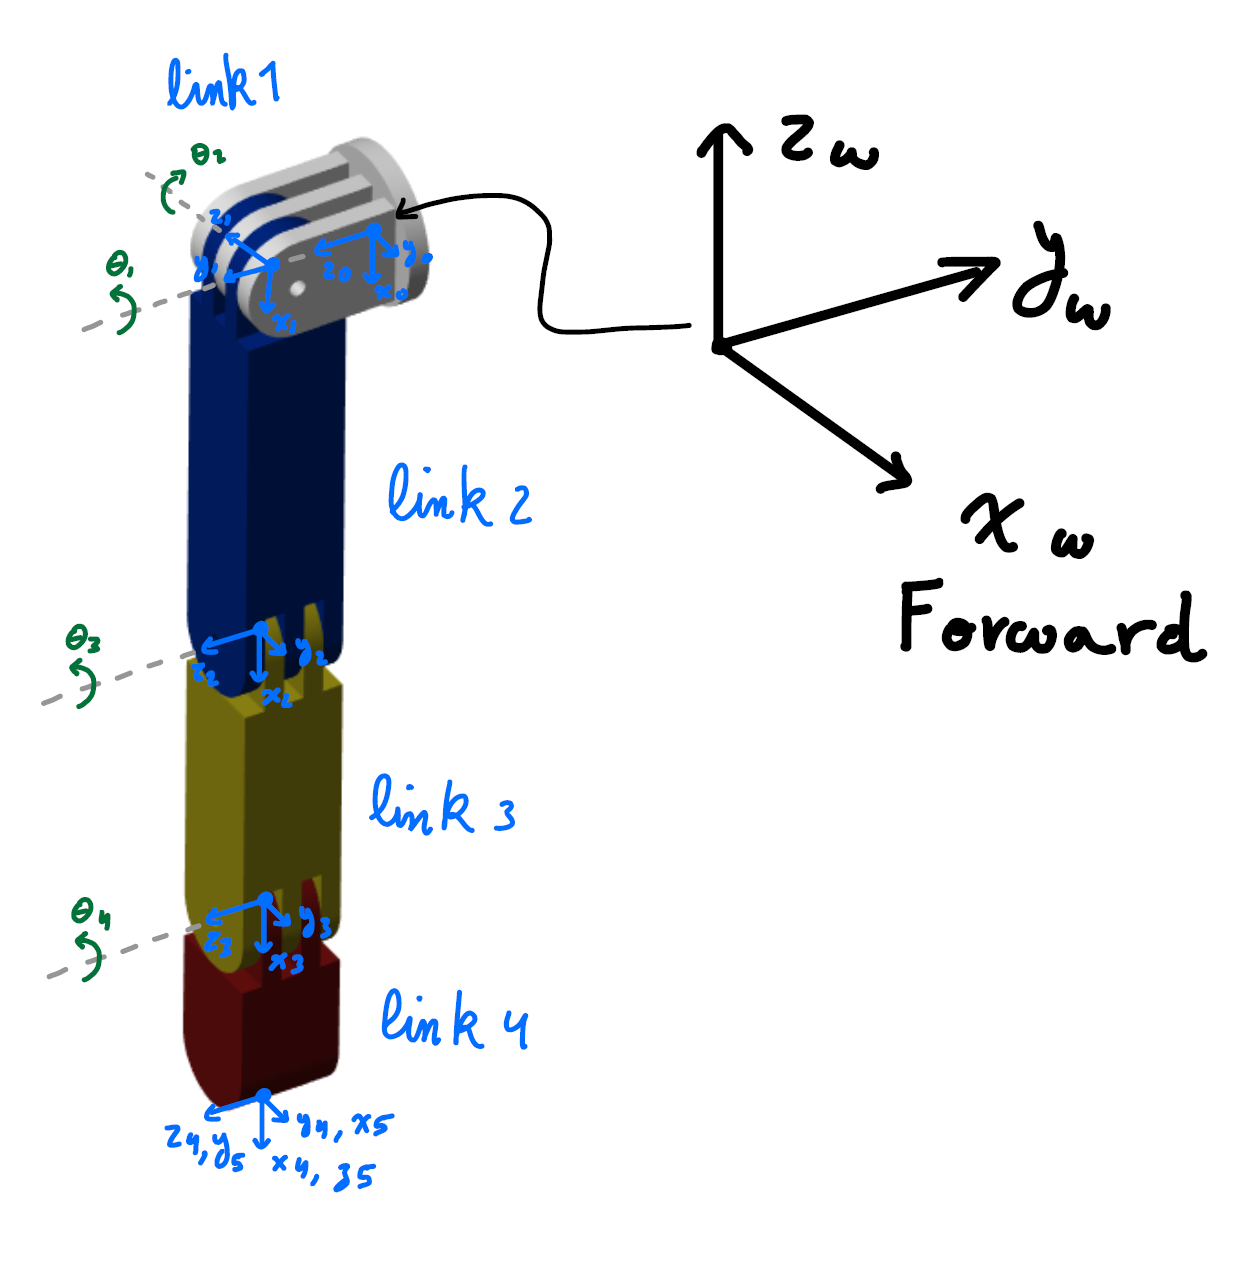
\includegraphics[width=\linewidth]{dhframes.png}}
    \caption{The chosen DH frames.}
    \label{fig:dhframes}
\end{figure}

The most important set of calculations is the DH-parameters. This computation is the precursor of all the work that follows in terms of forward kinematics and dynamic modeling. Since, in our model, all legs are designed to be similar, we only need to specify the DH-parameters for one leg. Figure \ref{fig:dhframes} shows the chosen frames. The rationale behind choosing the robot's frame $F_w$ as having the z-axis pointing upward as opposed to having it point in the direction of the axis of the first joint is to make subsequent computations of the dynamic model intuitive, especially when gravity is to be considered. This design choice gives us some sort of intuitive assumption that gravity points down by default (which will also be made to change with the orientation of the robot).
Table \ref{tab:dhparams} shows the DH-table that situates the frames with respect to the robot's world frame as shown in figure \ref{fig:dhframes}. The first two rows correspond to the transformation from the world frame to the first joint's frame, the next four are those that propagate the frame orientations based on the values of the joint angles, and the last one orients the approach vector along the final link's axis, which is customary to do, in the literature, and useful, in practice.

\begin{table}
\caption{DH-Parameters}
\label{tab:dhparams}
\begin{center}
\begin{tabular}{ | c | c | c | c | c |} 
\hline
link & $\theta_i$ & $d_i$ & $a_i$ & $\alpha_i$ \\
\hline
Rot1 & 0 & 0 & 0 & $\frac{\pi}{2}$ \\
\hline
Rot2 & $-\frac{\pi}{2}$ & 0 & 0 & 0 \\
\hline
1    & $\theta_1$ & 30  & 0  & $\frac{\pi}{2}$  \\
\hline
2    & $\theta_2$  & 0  & 100 & $-\frac{\pi}{2}$  \\
\hline
3    & $\theta_3$  & 0  & 75  & 0 \\
\hline
4    & $\theta_4$  & 0  & 50  & 0 \\
\hline
5    & $\frac{\pi}{2}$  & 0  & 0  &  $\frac{\pi}{2}$ \\
\hline
\end{tabular}
\end{center}
\end{table}

Figure \ref{fig:dhvalidation} shows how we validated those DH-parameters.

\begin{figure}[thpb]
    \parbox{\linewidth}{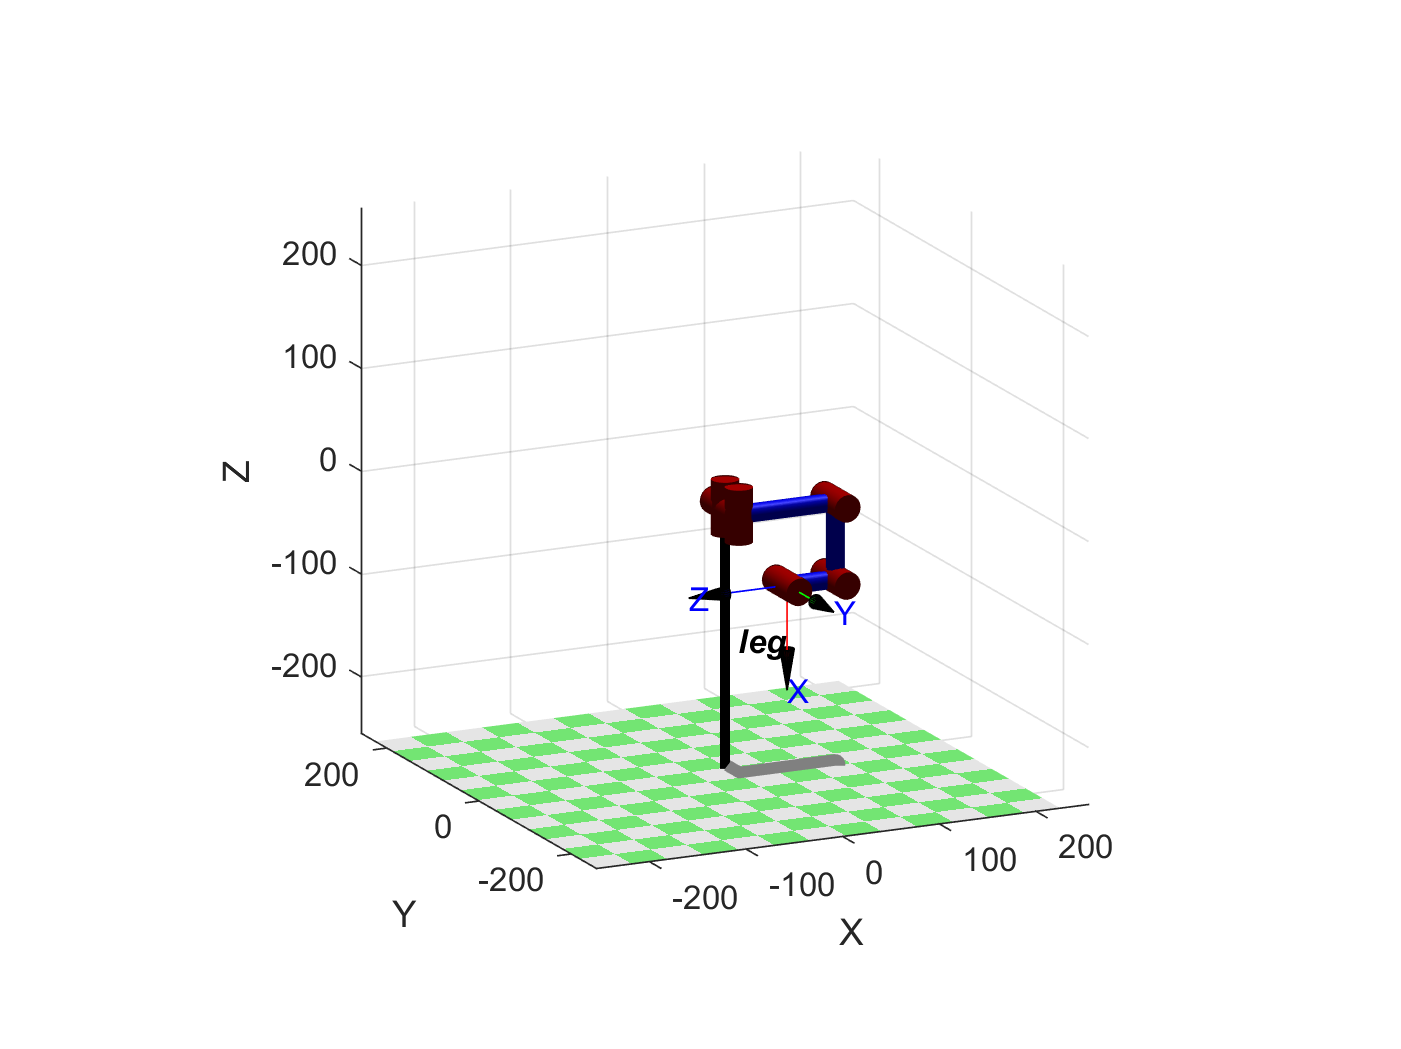
\includegraphics[width=\linewidth]{dhvalidation.png}}
    \caption{The plot that validates our DH-parameters. The configuration $\theta$ was set to [$\frac{\pi}{2}$ 0 -$\frac{\pi}{2}$ -$\frac{\pi}{2}$] to give the expected configuration in a plot. The Robotics Toolbox for MATLAB was used to generate this plot.}
    \label{fig:dhvalidation}
\end{figure}

\subsection{Forward Kinematics}
Given those DH-parameters shown in \ref{sec:dhparams}, it is almost trivial to compute the forward kinematics. A MATLAB function is setup for reuse across this project. The MATLAB function returns all the intermediate frames in a 3D matrix, for convenience and efficiency. This function will be used once in the Jacobian computation and the 3D matrix is used more than once, which removes the overhead due to calling this function and computing the forward kinematics.

\subsection{Inverse Kinematics}
At first we had decided to calculate the inverse kinematics using a geometric approach, and we actually did manage to do so. However, after doing some research, we decided to use a different approach. By calculating the inverse velocity kinematics, we can represent a trajectory in task-space, and interpolate the intermediate joint angles from there, as explained in \cite{spong2006robot}, and in Section \ref{sec:trajectories} Trajectories and Controller.


\subsection{The Jacobian}
The Jacobian of an individual leg is the single most important aspect in the process of dynamically modeling the quadruped in question. In fact, we need to be able to compute more than one Jacobian for each configuration, one for each link in the manipulator/leg.
For this purpose, we referred to the book "Robot Modeling and Control" \cite{spong2006robot}, which gives a cookbook method of computing the Jacobian for a point along one of the links of an n-link manipulator. Based on that, we created a function that takes the index of the joint and returns a corresponding 6x4 Jacobian matrix. For the purpose of dynamically modeling the robot, we do not need the matrix to be square. However, for the purpose of task-space trajectory tracking we need the pseudo-inverse.

\subsection{Dynamic Modeling}
From the process of dynamically modeling the robot, we computed the Lagrangian, as well as the inertia matrix and the potential energy matrix.
Thus far, we have a MATLAB script that outputs the inertia matrix and the potential energy vector of a specific configuration, what remains to be done is making the set of equations symbolic and doing the differentiations that the Euler Lagrange method requires.
However, we are expecting to get a slower version of the current code, which currently runs at 9 milliseconds (very good for control), because the symbolic library in MATLAB is known to be slow when used to compute the actual values through substitution. However, we still have to validate whether it does that or not.
After we do the differentiation, we get the equations of motion that should allow us to figure out the torques required to fight off gravity, for example.
\subsubsection{The System's Lagrangian}
We referred to \cite{spong2006robot} for the process of computing the total energy of the system, kinetic and potential. This allowed us to use the Euler-Lagrangian equations of motion that are essential to perform gravity compensation and other dynamic terms cancellation that are needed when we use computed torque control, as a way to control the robot and have it follow trajectories.
We were able to compute or acquire the matrices that define the following, so called inertia matrix, as defined in \cite{spong2006robot}.
$$
M(q) = \sum_{i=1}^n \{m_i J_{vi}(q)^T J_{vi}(q) + J_{\omega i}(q)^T R_i(q) I_i R_i(q) J_{\omega i}(q)\}
$$
The total kinetic energy of the system can be computed using the following equation:
$$
k = \frac{1}{2} \dot{q}^T M(q)\dot{q}
$$
where i is in the index of the center of mass of the $i^{th}$ link, $J_{vi}$ the linear velocity part of the Jacobian, and  $J_{\omega i}$ the rotational part of it for the center of mass of the $i^{th}$ link.
The total potential energy in the system is defined as follows.
$$
P = \sum_{i=1}^n  m_i g^T r_{ci}
$$
where $r_{ci}$ is the location of the center of mass of the $i^{th}$ link and $m_{ci}$ is the mass thereof. g in here is the orientation of the gravity vector. This is what we are planning to change to accommodate the model to different base orientations when the robot is walking.

\section{ENVISIONED APPROACH}
The process that we envision is the following. After getting the dynamic model of a leg of the robot
$$
\tau = M(q)\ddot{q} + C(q,\dot{q})\dot{q} + G(q),
$$ we can extend that model in two ways.
First, we either maintain world to leg frame transformation that we update using our measurements (prone to error in the real world), or recompute from scratch the equations and change the gravity vector to reflect the new orientation of the body which we can readily measure using an IMU assumed to be on-board (like proprioception that humans have). We may also parameterize the gravity vector to include those measurements. Independent from this model we may maintain position, and velocity (linear and rotational) variables for the whole system, as prescribed in \cite{hardt2003dynamic}. However, our aim is to make the robot walk a few steps as opposed to being provably stable, so whatever gets us to make the robot walk as a reach goal, we will undergo.

\subsection{Trajectories and Controller} \label{sec:trajectories}
This model will then be used in a computed torque controller to make the leg faithfully follow the trajectories we specify. While MATLAB allows us to do position-based control, we will refrain from using that feature, as this is not the case with real-robots.

As for trajectory generation, we will generate these in the task-space as opposed to the joint-space. For that, we do not need any inverse kinematics, only inverse velocity kinematics. From the reference book \cite{spong2006robot}, we can represent the trajectory-to-follow in the task-space and get its equivalent trajectory in the joint-space.
Given the following equations, we can do the translation.
$$
\dot{X} = J_a(q)\dot{q} 
$$
$$
\ddot{X} = J_a(q)\ddot{q} + \dot{J_a}(q)\dot{q}
$$
$$
\ddot{q} = a_q
$$
By defining $a_q$ as $J^{-1}\{a_X - \dot{J}\dot{q}\}$, we can can then directly command the acceleration, as can be seen in the resulting equation $\ddot{X} = a_X$. Then, we can track the trajectory using a PD controller with feed-forward like so:
$$
a_X = \ddot{X}^d - k_p (X - X^d) - k_d (\dot{X} - \dot{X}^d)
$$
Thus, by computing the desired acceleration at the joint level using $a_q = J^{-1}\{a_X - \dot{J}\dot{q}\}$, we can track a trajectory in task-space. In here, the task space is considered with respect to the frame of the leg, as shown in figure \ref{fig:dhframes}.

\subsection{Central Pattern Generator}
As per the work in \cite{kimura2007adaptive}, we will use the concept of a central pattern generator. Once we have the trajectories, which can be systematically generated or specified manually (engineered), we can create a simple central pattern generator, a higher-level controller that regulates the phase between the trajectories that the legs follows (the same trajectory for all legs), possibly with some minor changes to angle signs.

A simple approach to the central pattern generator would simply regulate the difference between $t_1$, $t_2$, $t_3$, and $t_4$, such that $0 < t_1 < t_2 < t_3 < t_4 < T$ where T is the final time of the trajectory, and each of those time variables corresponds to the progress of the respective leg along its trajectory.

\subsection{Assumptions Taken}
One important consequence of our modeling approach is that we are treating the weight of the body as a disturbance, by virtue of the choice of modeling each leg independently. This means that we are also assuming that we can measure the forces at the leg that are generated by the weight of the body very accurately and separate it out from the weight of the leg (which we can do since we are modeling it's weight).
We are also assuming that we can measure the legs configurations in terms of position and velocity.

% \section{Hypothesis}
% As we were thinking of the different ingredients to our rather simple method of making the robot walk, a hypothesis was brewing in our minds. \\
% \textbf{Hypothesis:} The robot, augmented with the above modeling and compensation, will be able to stand, and perform a few steps on a smooth plane before stumbling.

\section{Challenges}
Like any project, we ran into a few major issues that slowed our progress more than expected. The first of these problems were our 4 DoF leg. Unlike most quadrupeds, our leg design has a single roll joint, with a planar 3DoF manipulator. This configuration allows us to have nearly unlimited attack angles to the ground, but also introduces a lot of complexity when calculating inverse kinematics and modeling the dynamics of the leg.

We also ran into problems when dynamically modeling the legs themselves. No group member had experience in dynamic modeling, so we studied literature and asked professors to learn how dynamic modeling worked in a case like ours. We also simplified the model (see Section \ref{sec:CAD Model Design}), to make the modeling process easier.

Our final major problem we faced was our inexperience with MATLAB SimMechanics modeling. This inexperience led to many refactors of our code base, and although another refactor may happen in the near future, we think that our software is at a point where we can continue development with less distractions.

\section{PROJECT PLAN}
\subsection{Updated Schedule}
    \begin{figure}[thpb]
        \parbox{\linewidth}{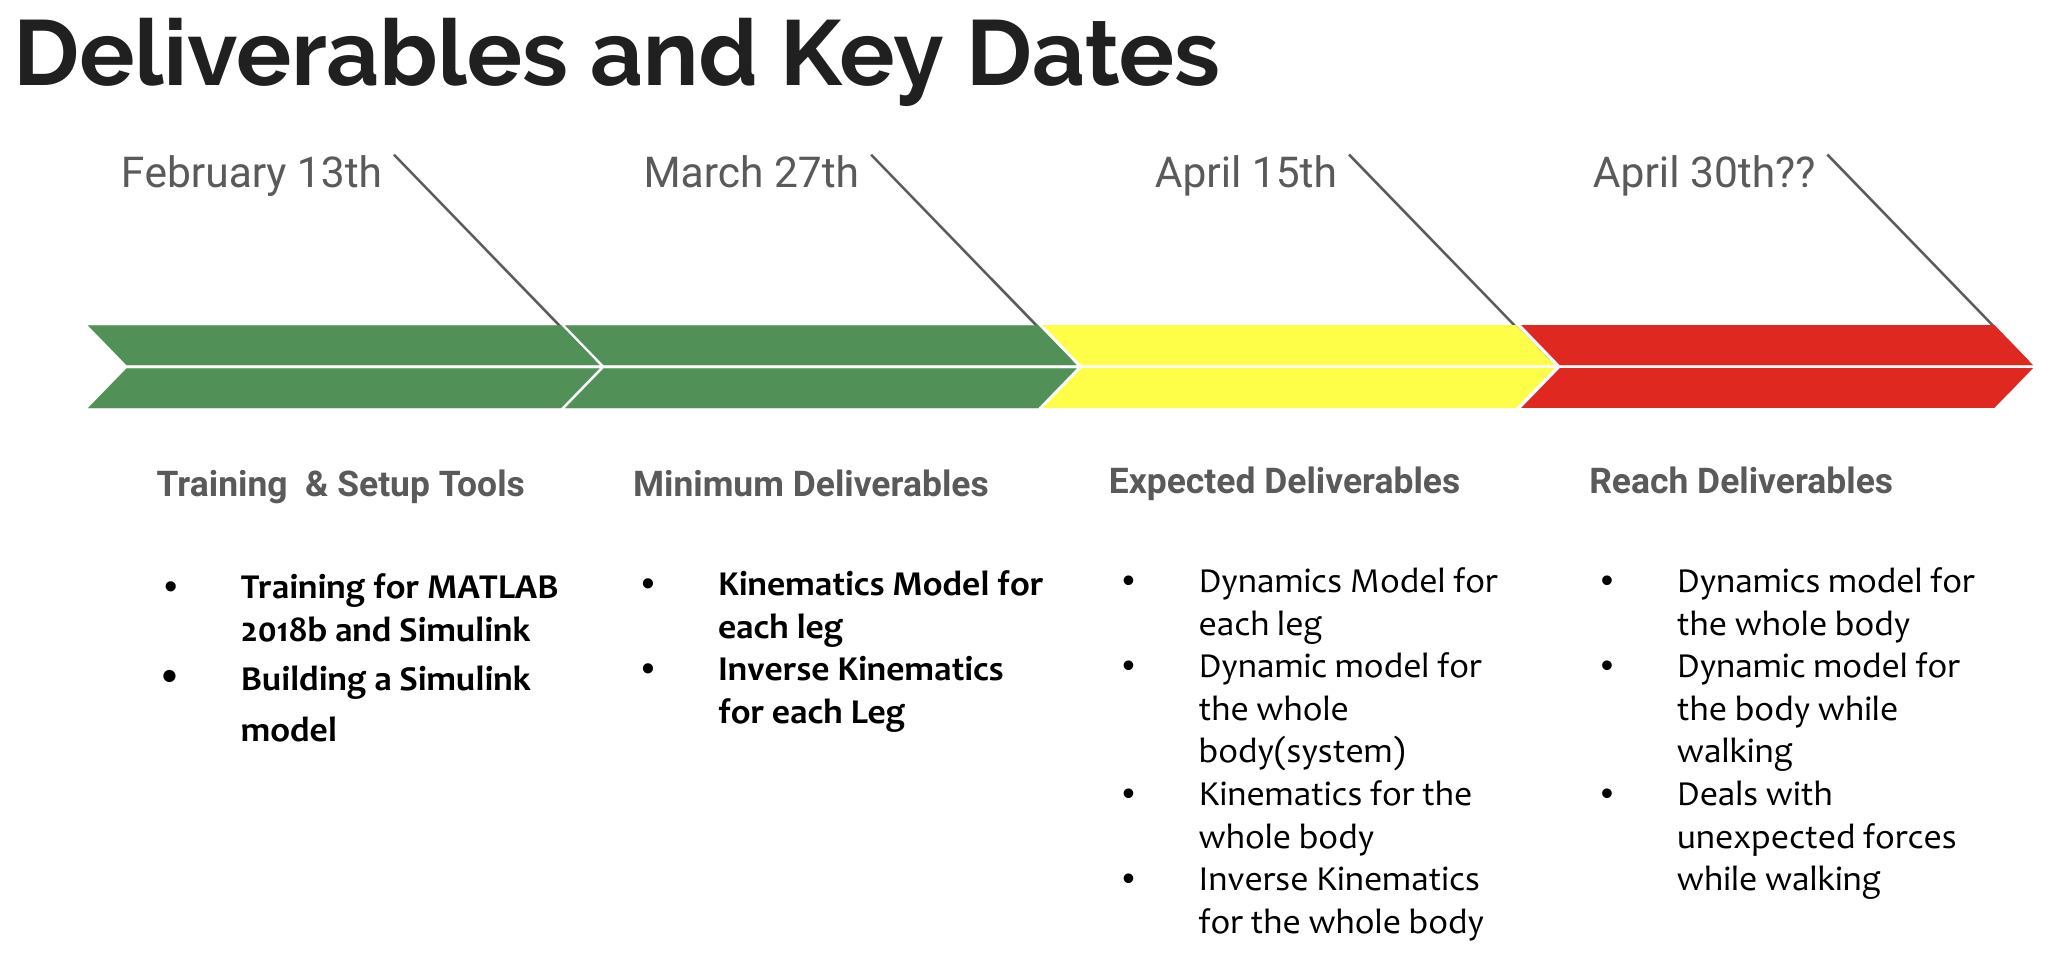
\includegraphics[width=\linewidth]{UpdatedSchedule.png}}
        \caption{Our updated schedule. Bolded tasks have been completed}
        \label{fig:updatedschedule}
    \end{figure}
\subsection{Dependencies}
We have two major dependencies coming into the second half of our project: our dynamic model for our leg and our dynamic model for our body. As seen in the schedule, we want to not only model our quadruped, but also give it basic control over its body. This will require a bullet proof model for each leg, which will be used for a dynamic body model. Although this is our reach goal, we hope to finish it within the next few weeks, and to have a demo ready.

\section{CONCLUSION}
Although we are on track with our original estimation, our team would like to be further ahead than we are. However, the steps we have taken to learn key concepts and develop good code has put us in a position that will hopefully expedite our future endeavours in our project. We are excited to see if our modeling approaches will allow us to achieve a torque controlled dynamic walking robot. If successful, this may provide a decent method to model and control commercial grade walking quadrupeds, and allow for more advanced stability studies and improvements to the controller.

\addtolength{\textheight}{-12cm}   % This command serves to balance the column lengths
                                  % on the last page of the document manually. It shortens
                                  % the textheight of the last page by a suitable amount.
                                  % This command does not take effect until the next page
                                  % so it should come on the page before the last. Make
                                  % sure that you do not shorten the textheight too much.

% \section*{APPENDIX}

% Appendixes should appear before the acknowledgment.

\section*{ACKNOWLEDGMENT}

\bibliographystyle{plain} % We choose the "plain" reference style
\bibliography{references} % Entries are in the "refs.bib" file

\end{document}
